\chapter{Background theory}\label{chapter:theory}

This chapter introduces relevant kinematics, dynamics and control for the snake robot specific case used in the development of the simulator. Further, the concepts of OAL and HPFC are explained to give insight into the motivation and structure of the simulator. Even though the idea of dynamical HPFC \cite{yoshikawa1987dynamic} is not applied in the project, it is presented as it is an essential part of the discussions in Chapter \ref{ch:discussion}. Lastly, the methods for detecting contact with obstacles and adjusting to a predefined path are explained.


\section{Snake robot kinematics}\label{sec:kin}


The snake robot is modeled as a serial chain, which is a system of rigid bodies in which each member is connected to two others, except for the first and last members that are each connected to only one other member \cite{waldron2016kinematics}. As opposed to traditional robot manipulator models, the first joint in the snake robot model is not physically connected to a base.


The vector of generalized coordinates $\mathbf{q}$ for a snake robot with $n$ links is

\begin{equation} \label{eq:q}
    \mathbf{q} = 
    \begin{bmatrix}
        \phi_1 & \phi_2 & ... & \phi_n & x_0 & y_0
    \end{bmatrix}^T.
\end{equation}
\\
The coordinates $(x_0, y_0)$ and $\phi_1$ represent the position and orientation of the tail of the snake robot in reference to the base frame $(x,y)$. These coordinates cannot be directly controlled and will therefore be referred to as virtual coordinates. The generalized coordinates ${\phi_2, ... ,  \phi_n}$, corresponding to the actuated joints, refer to the angle of the following link relative to the preceding link. The number of generalized coordinates including two position coordinates and $n$ joint angles is $N = n+2$.

The model of the snake robot with the named variables are illustrated in Figure \ref{fig:kin_name}. 
\begin{figure}
    \centering
    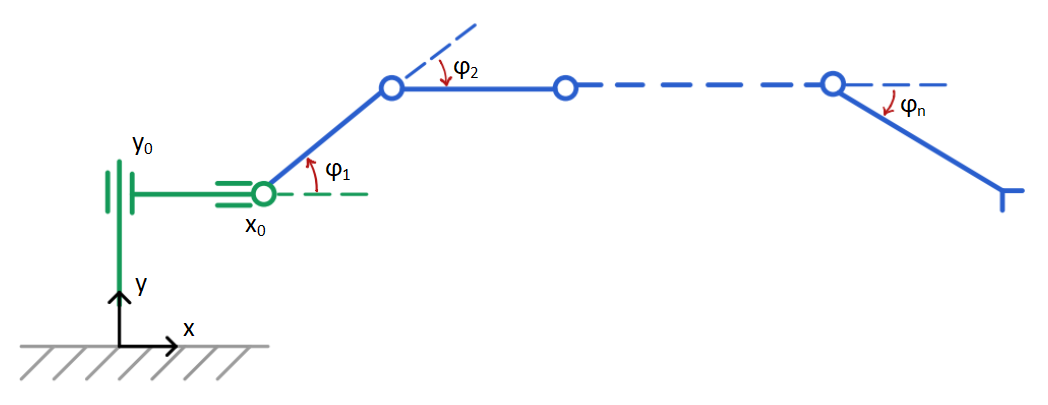
\includegraphics[width=0.9\textwidth]{figures/kinematics.PNG}
    \caption{Model of snake robot with notation}
    \label{fig:kin_name}
\end{figure}


Homogeneous transformation matrices are used to express the pose (position and orientation) of the links in relation to the base frame. This means that as long as the joint angles and size of the snake robot are known, the Cartesian positions can be calculated.
The homogeneous transformation matrix for the end point of link $i$ from the base frame $b$ is given by (\ref{eq:transformationmatrix}). The base frame will stay put regardless of motion of the robot. Note also that the link length $l$ is assumed equal for all the links.

\begin{equation} \label{eq:transformationmatrix}
    \textbf{T}_{b i} = \textbf{D}_x(x_0) \textbf{D}_y(y_0) \sum_{k=1}^{i} \textbf{R}_z(\phi_k) \textbf{D}_x(l)
\end{equation}
\\
The translation and rotation matrices are given by

\begin{equation}\label{eq:trans_rot}
    \begin{split}
        \textbf{D}_x(x)& = 
        \begin{bmatrix}
            1 & 0 & x \\
            0 & 1 & 0 \\
            0 & 0 & 1
        \end{bmatrix}, \ \
        \textbf{D}_y(y) =
        \begin{bmatrix}
            1 & 0 & 0 \\
            0 & 1 & y \\
            0 & 0 & 1
        \end{bmatrix}, \ \
        \\&
        \\&\textbf{R}_z(\phi) =
        \begin{bmatrix}
            \cos{\phi} & -\sin{\phi} & 0 \\
            \sin{\phi} &  \cos{\phi} & 0 \\
            0          &  0          & 1
        \end{bmatrix}.
    \end{split}
\end{equation}
\\
The transformation matrix from the reference frame to the center of link $i$ can be found in the same manner. The only difference is that the very last translational matrix has to take the argument $l/2$ instead of $l$. This is useful to keep in mind as it be used in Section \ref{sec:dyn} for the derivation of the kinetic energy of the links.

As mentioned earlier, the transformation matrix $\textbf{T}_{b i}$ can be used to find the absolute orientation and position of the tip of link $i$ in the base frame.
The resulting matrix can be written on the form

\begin{equation}
    \textbf{T}_{b i} =
    \NORMAL{
    \begin{bmatrix}
        \textbf{R}_{b i}(\phi_{i,abs}) & \textbf{t}_{r i}^r \\
        \textbf{0}^T & 1
    \end{bmatrix} }.
\end{equation}
\\
The position is directly extracted from $\textbf{t}_{r i}^r = [x_i y_i]^T$. The orientation $\phi_{i,abs}$ is found by comparing $\textbf{R}_{b i}$ to $\textbf{R}_z$ and solving for $\phi_{i,abs}$.

Alternatively, one can directly compute the position of the center of a link $i$ from the expressions below

\begin{equation} \label{eq:pos}
    \begin{split}
        x_i &= x_0 + \sum_{k=1}^{i} l \cos{(\sum_{j=1}^{k} \phi_j)} \\
        y_i &= y_0 + \sum_{k=1}^{i} l \sin{(\sum_{j=1}^{k} \phi_j)},
    \end{split}
\end{equation}
\\
where $l$ is the link length and $1\leq i\leq n$.

\subsubsection{Forward and inverse instantaneous kinematics}\label{subseq:inst_fwd}

The well known Jacobian lets us transform between Cartesian and joint velocities. It is derived by taking the partial derivative of the $x$ and $y$ position of link $1\leq i\leq n$ with respect to all generalized coordinates

\begin{equation}\label{eq:Jc1}
    \mathbf{J_i} = 
    \HUGE{
    \begin{bmatrix}
        \frac{\partial x_i}{\partial q_1} & ... & \frac{\partial x_i}{\partial q_{N-1}} & \frac{\partial x_i}{\partial q_{N}} \\
        \frac{\partial y_i}{\partial q_1} & ... & \frac{\partial y_i}{\partial q_{N-1}} & \frac{\partial y_i}{\partial q_{N}} \\
    \end{bmatrix}
    }.
\end{equation}
\\
The relationship between the Cartesian velocity $\mathbf{v}$ of the point $(x_i, y_i)$ on the robot and the joint velocities $\mathbf{\dot{q}}$ can thus be written as 

\begin{equation}
    \mathbf{v_i = J_i(q) \dot{q}} \quad \textrm{ and } \quad \mathbf{\dot{q} = J_i(q)^\dagger v_i}.
\end{equation}
\\
The first equation is formally referred to as the forward instantaneous kinematics, whereas the second one is referred to as the inverse instantaneous kinematics.
$\mathbf{J(q)^\dagger}$ is the pseudo inverse of the Jacobian, which has to be used as a result of the Jacobian being non-square.

%------------------------------------------------------------------------------------------------

\subsection{Constrained kinematics}\label{seq:constr_kin}

%\hl{Virtual closed kinematic chain}\\
For the case in which the robot is in contact with the environment, the motion will be constrained. The obstacles found in the environment are modelled as single frictionless points. The only constraint imposed by the environment is that the robot cannot penetrate the obstacles. It can, however, both apply an arbitrary large force against them or move along them.

The model assumes that any link can be in contact with at most one obstacle at the time. To represent the mentioned constraint, the vector of generalized coordinates is expanded with $n$ further elements, where $n$ is the number of links. The updated vector $\mathbf{q}$ is now

\begin{equation} \label{eq:q2}
    \mathbf{q} = 
    \begin{bmatrix}
        \phi_1 & \phi_2 & ... & \phi_n & x_0 & y_0 & d_{c,1} & d_{c,2} & ... & d_{c,n}
    \end{bmatrix}^T,
\end{equation}
\\
where $N = 2 + 2n$ is the new number of generalized coordinates.

The newly introduced coordinates $d_{c,1}, ... , d_{c,n} \geq 0$ represent the distance to the possible contact point from the corresponding joint. For instance, the coordinate $d_{c,2}$ is the distance between the second joint and the contact point measured along the second link, as illustrated in Figure \ref{fig:3_obs_force}. Every link might not be in contact with an obstacle, but the maximum number of coordinates is introduced in the interest of keeping the vector size constant. 
Seeing as there is no actuation force directly connected to the obstacle-related coordinates, they will be referred to as virtual joints or virtual coordinates.

The position of a contact point on link $1\leq i\leq n$ in the base frame can be derived through the corresponding transformation matrix (\ref{eq:obst_tfmatrix}).

\begin{equation} \label{eq:obst_tfmatrix}
    \textbf{T}_{b ci} = \textbf{D}_x(x_0) \textbf{D}_y(y_0) \sum_{k=1}^{i-1} (\textbf{R}_z(\phi_k) \textbf{D}_x(l)) \textbf{R}_z(\phi_i) \textbf{D}_x(d_{c,1})
\end{equation}

\begin{figure}
    \centering
    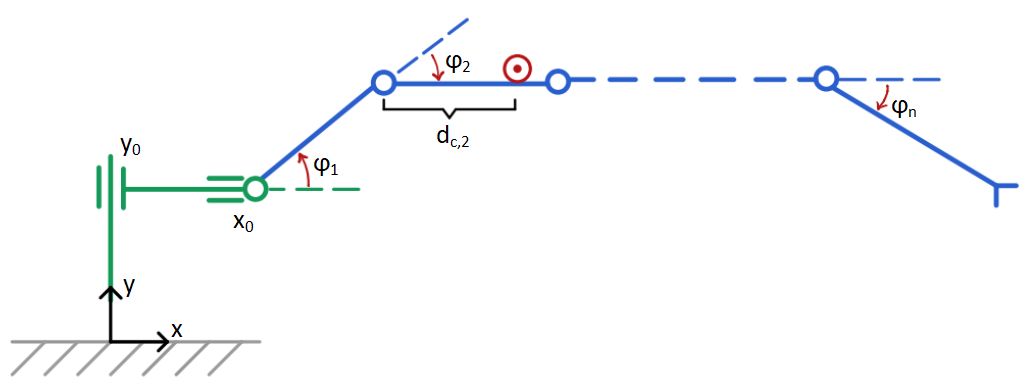
\includegraphics[width=0.9\textwidth]{figures/contact_point.PNG}
    \caption{Snake robot in contact with obstacle}
    \label{fig:3_obs_force}
\end{figure}


%------------------------------------------------------------------------------------------------

\subsubsection{Constrained instantaneous kinematics}\label{subseq:constr_inst}

The Jacobian matrix related to the velocity of the contact point can be derived in the same manner as in the unconstrained case. The only difference is that the partial differentiation of the contact point $(x_c,y_c)$ is now taken with respect to the extended vector of generalized coordinates (\ref{eq:q2}). The resulting contact Jacobian for a contact point on link $1\leq i\leq n$ is thus

\begin{equation}\label{eq:Jac_constr}
    J_{c,i} = 
    \HUGE{
    \begin{bmatrix}
        \frac{\partial x_{c,i}}{\partial \phi_2} & ... & \frac{\partial x_{c,i}}{\partial q_{N-1}} & \frac{\partial x_{c,i}}{\partial q_N} \\
        \frac{\partial y_{c,i}}{\partial \phi_2} & ... & \frac{\partial y_{c,i}}{\partial q_{N-1}} & \frac{\partial y_{c,i}}{\partial q_N} \\
    \end{bmatrix}
    }.
\end{equation}
\\
This Jacobian will end up being quite sparse, seeing as the coordinate of a contact point is independent of all other contact coordinates. This is a property that can be exploited using sparse solvers if the snake robot has a large number of links.

The relationships between the Cartesian velocity of a contact point on link $1\leq i\leq n$ and the joint velocities can now be expressed as

\begin{equation}
    \mathbf{v_{c,i} = J_{c,i}(q) \dot{q}} \quad \textrm{ and } \quad \mathbf{\dot{q} = J_{c,i}(q)^\dagger v_{c,i}}.
\end{equation}


%------------------------------------------------------------------------------------------------
%------------------------------------------------------------------------------------------------

\section{Snake robot dynamics} \label{sec:dyn}

The snake robot has $n-1$ joint actuators that all can apply torques to their corresponding joints. The dynamics describe how the robot moves in response to these actuator forces. For simplicity, it is assumed that the actuators do not have dynamics of their own and, hence, arbitrary torques can be commanded at the joints of the robot \cite{murray2017mathematical}.

The dynamics of the snake robot will be expressed using the joint space equations of motion formulation

\begin{equation}
    \mathbf{M(q)\ddot{q} + C(q, \dot{q}) + g(q)} = \boldsymbol{\tau}.
\end{equation}
\\
Because the movement is restricted to the 2D plane, the gravitational term $\mathbf{g(q)}$ can be neglected and the equations of motion can be rewritten to

\begin{equation}\label{eq:eom}
    \mathbf{M(q)\ddot{q} + C(q, \dot{q})} = \boldsymbol{\tau},
\end{equation}
\\
where $\mathbf{M(q)}$ and $\mathbf{C(q,\dot{q})}$ is the mass matrix and Coriolis matrix respectively.
$\boldsymbol{\tau}$ is the vector of generalized torques corresponding to the generalized coordinates (\ref{eq:q}). Furthermore, the elements corresponding to the virtual coordinates will be zero at all times.

Solving (\ref{eq:eom}) with respect to $\mathbf{\ddot{q}}$ yields

\begin{equation}\label{eq:eom_qdd}
    \mathbf{\ddot{q}} = \mathbf{M^{-1}(q)}( \boldsymbol{\tau} - \mathbf{C(q, \dot{q})}).
\end{equation}
\\
Several methods exist for finding the equations of motion for a robot. The Euler-Lagrange method \cite{lynch2017modern}, which  is chosen here, is based on the difference in kinetic energy ($K$) and potential energy ($P$) of the system, also known as the Lagrangian

\begin{equation}
    L = K - P.
\end{equation}
\\
The equations of motion can now be expressed as a second order partial differential equation

\begin{equation} \label{eq:Lagrange}
    \frac{d}{d t} \frac{\partial L}{\partial \mathbf{\dot{q}}} - \frac{\partial L}{\partial \mathbf{q}} = \boldsymbol{\tau}.
\end{equation}
\\
Again, simplifications can be made from the restricted movement in the world and thus the potential energy $P$ can be neglected. The Lagrangian is therefore simply equal to the kinetic energy, which is the sum of the kinetic energy for every link \cite{rezapour2014path}. Furthermore, the kinetic energy for one link $i$ is divided into two parts, $K_{translational}$ and $K_{rotational}$.
The kinetic energy can now be express as

\begin{equation}\label{eq:kinen}
    K = \sum_{i=1}^{n} (K_{translational,i} + K_{rotational,i}),
\end{equation}
\\
where the translational and rotational kinetic energy is given in (\ref{eq:k_trans}) and (\ref{eq:k_rot}) respectively.

\begin{equation} \label{eq:k_trans}
    K_{translational,i} = \frac{1}{2} m (\dot{x}_i^2 + \dot{y}_i^2)
\end{equation}
\\
Here $m$ is the link mass, and $(\dot{x}_i, \dot{y}_i)$ make out the velocity of the center of the link found by differentiating (\ref{eq:pos}) with respect to time. 

\begin{equation} \label{eq:k_rot}
    K_{rotational,i} = \frac{1}{2}I\dot{\phi_i}^2
\end{equation}
\\
$\dot{\phi}_i$ is the joint velocity of link $i$. Furthermore, every link has the same moment of inertia, namely $I = (1/12)ml^2$. This is the moment of inertia of a rod, corresponding to the moment of inertia of a cylinder with zero radius \cite{lynch2017modern}.


%------------------------------------------------------------------------------------------------

\subsection{Constrained dynamics}\label{subseq:constr_dyn}

The generalized torques from the right side of (\ref{eq:eom}) can be split into two parts whenever there is contact between the robot and the environment, namely a component resulting from the control inputs (motor torques), $\boldsymbol{\tau_{m}}$, and a component resulting from the external forces acting on the robot, $\boldsymbol{\tau_{c}}$ \cite{rezapour2014path}. The generalized torques can thus be written

\begin{equation}
    \boldsymbol{\tau} = \boldsymbol{\tau_{m}} + \boldsymbol{\tau_{c}}.
\end{equation}
\\
According to Holden et al. \cite{holden2014optimal}, the force from an obstacle acting on a link is two-fold: one normal to the link and one tangent to the link. The force tangent to the link is due to friction and will therefore be neglected in this project. The remaining normal force is preventing the link from moving into the obstacle when the robot itself is applying a force to the obstacle. The external force in the frame of link $i$ acting on link $i$ is denoted $\mathbf{f}^i_{c,i}$ and can be written as

\begin{equation}
    \mathbf{f}^i_{c,i}=
    \begin{bmatrix}
        0 \\
        f^i_{c,i,y}
    \end{bmatrix}.
\end{equation}
\\
The following derivations are inspired by \cite{rezapour2014path}. The force $\mathbf{f}^i_c$ can be expressed in the base frame by using the rotation matrix from (\ref{eq:trans_rot}):

\begin{equation}
    \mathbf{f}^b_{c,i} = \mathbf{R}_z(\alpha_i) \mathbf{f}^i_{c,i},
\end{equation}
\\
where $\alpha_i$ is the angle of link $i$ related to the base frame $b$. It can be found by 

\begin{equation}
    \alpha_i = \sum_{k=1}^{i} \phi_k.
\end{equation}
\\
The contact Jacobian (\ref{eq:Jac_constr}) can be used to find the generalized external torque as a result of the external forces:

\begin{equation}\label{eq:tauforcerel}
    \boldsymbol{\tau_c} = \sum_{i=1}^{n} \mathbf{J}^T_{c,i} \mathbf{f}^b_{c,i}.
\end{equation}



%------------------------------------------------------------------------------------------------
%------------------------------------------------------------------------------------------------

%\section{Obstacle contact force}



%The force the obstacle is pushing back with on link $m$ is simply denoted , where $\mathbf{\norm{f_m} = \norm{f_{c,m}}}$. The sign of the force will also depend on which side of the link the obstacle is lying on \cite{holden2014optimal}. The sign is here denoted by $\gamma_m$, where $\gamma_m > 0$ for obstacles to the right of the link and vice versa. The force acting on link $m$ is thus

%The different forces acting on the robot can be stacked in the matrix $\mathbf{F_m}$ and the corresponding transposed Jacobians can be stacked in the matrix $\mathbf{J_c}$. When all the forces from the different obstacles are found, the corresponding torques can be added to the equations of motion to obtain the resulting behavior of the robot. The updated equations of motion are

%The joint torque $\boldsymbol{\tau}$ from the robot is now acting on both the joints of the robot and on the obstacle. From basic physics theory we know that for rigid bodies, the force between two bodies are equal opposites. This means that the robot joint torque $\boldsymbol{\tau}$ has a component which will be cancelled by the obstacle force/torque. We call this component $\boldsymbol{\tau}_c$. The remaining torque $\boldsymbol{\tau_a}$ will contribute to accelerating the links of the robot. Hence, we can express the joint torque on the format


%------------------------------------------------------------------------------------------------
%------------------------------------------------------------------------------------------------

\section{Computed torque control}
The content of this section is taken from Chapter 11 of Modern Robotics \cite{lynch2017modernCompTorque}.

\subsection{PD control}
A common feedback controller is linear proportional-derivative control, or PD-control:

\begin{equation}\label{eq:pd}
    \boldsymbol{\tau} = \mathbf{K_p q_e + K_d \dot{q}_e}.
\end{equation}
\\
The control gains $\mathbf{K_p}$ and $\mathbf{K_d}$ are positive diagonal matrices. The proportional gain $\mathbf{K_p}$ acts as a virtual spring that tries to reduce the position error $\mathbf{q_e = q_d - q}$, where $\mathbf{q_d}$ is the desired joint angles. The derivative gain $\mathbf{K_d}$ acts as a virtual damper that tries to reduce the velocity error $\mathbf{\dot{q}_e = \dot{q}_d - \dot{q}}$.

Substituting the PD control law into the dynamics (\ref{eq:eom}) yields

\begin{equation}\label{eq:control1}
    \mathbf{M \ddot{q} + C(q, \dot{q}) = K_p (q_d - q) + K_d (\dot{q}_d - \dot{q})}.
\end{equation}
\\
The damping ratio $\zeta$ and natural frequency $\omega_n$ of this system is given as:

\begin{equation}\label{eq:control2}
    \zeta = \mathbf{\frac{K_d}{2 \sqrt{K_p M(q)}}} \quad  \
    \textrm{and} \quad \
    \omega_n = \mathbf{\sqrt{\frac{K_p}{M(q)}}}.
\end{equation}
\\
$\zeta = 1$ yields a critically damped behaviour, while larger values yield an overdamped behaviour. Furthermore, $\mathbf{K_p}$ should be chosen as high as possible if fast response is desired.

\subsection{Feedforward control}
%(Modern Robotics 11.4.1.2)\\
Another strategy for trajectory following is to use the model of the robot's dynamics (\ref{eq:eom}) to proactively generate torques instead of waiting for errors. The feedforward torque is calculated as 

\begin{equation}\label{eq:feedforward}
    \boldsymbol{\tau} = \mathbf{\Tilde{M}(q_d)\ddot{q}_d + \Tilde{C}(q_d, \dot{q}_d)},
\end{equation}
\\
where the model is perfect if $\mathbf{\Tilde{M}(q) = M(q)}$ and $\mathbf{\Tilde{C}(q,\dot{q}) = C(q,\dot{q})}$.


\subsection{Feedforward and feedback linearization} \label{subsec:comp_torque}
%(Modern Robotics 11.4.1.3) \\

As no model of the robot and environment will be perfect, it is not sufficient to use pure feedforward control. Combining the PD controller (\ref{eq:pd}), with a proper choice of PD gains, and a feedforward term (\ref{eq:feedforward}) will ensure exponential decay of the trajectory error (not just setpoint error).

Since $\mathbf{\ddot{q}_e = \ddot{q}_d - \ddot{q}}$,

\begin{equation}\label{eq:qdd}
    \mathbf{\ddot{q} = \ddot{q}_d + K_d \dot{q}_e + K_p q_e}.
\end{equation}
\\
Substituting (\ref{eq:qdd}) into the robot dynamics (\ref{eq:eom}) gives the computed torque controller, also known as feedforward plus feedback linearizing controller:

\begin{equation}\label{eq:controllaw}
    \boldsymbol{\tau} = \mathbf{\Tilde{M}(q) (\ddot{q}_d + K_d \dot{q}_e + K_p q_e) + \Tilde{C}(q,\dot{q})}.
\end{equation}
\\
A block diagram of the resulting control (\ref{eq:controllaw}) is shown in Figure \ref{fig:block-diag-torque}.

\begin{figure}
    \centering
    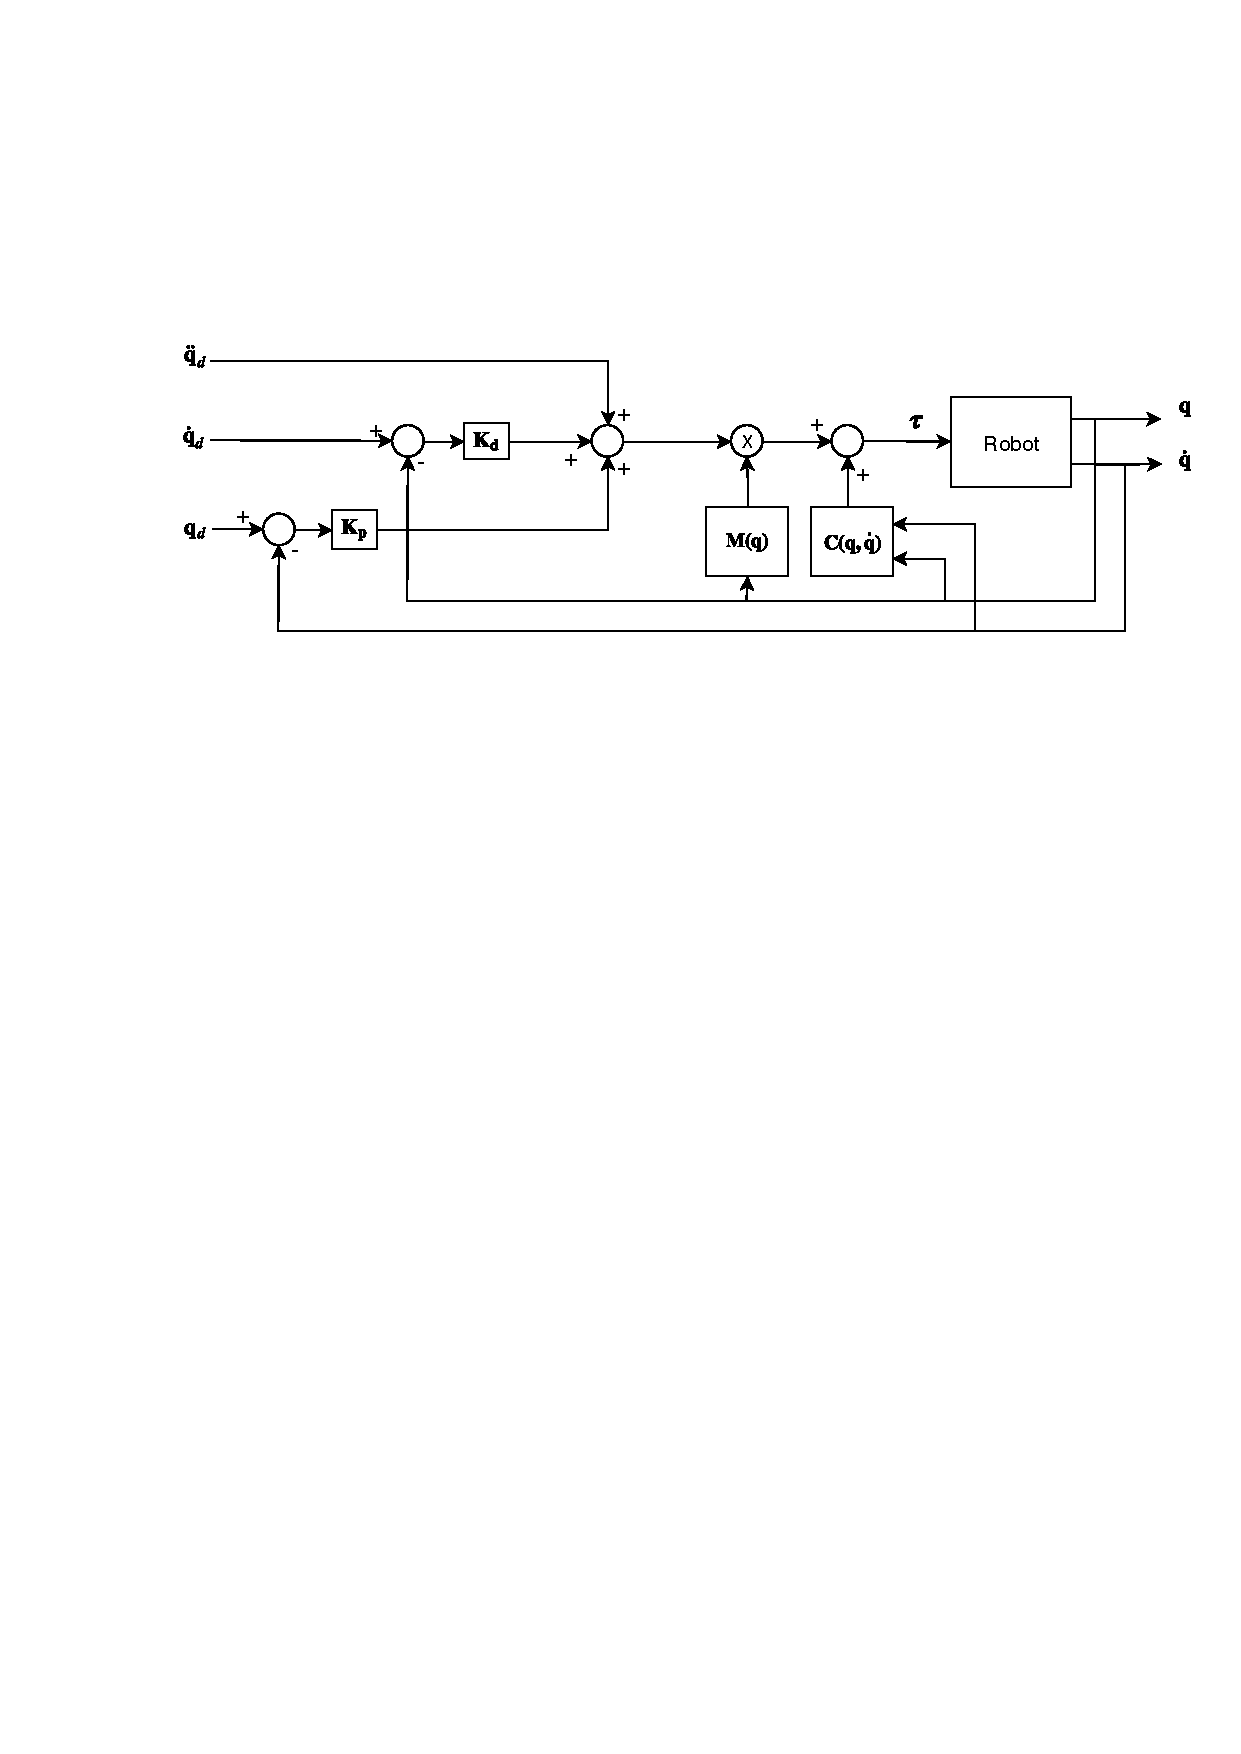
\includegraphics[trim=3cm 19cm 0.5cm 5cm, clip=true, width=0.9\textwidth]{figures/blockdiag.pdf}
    \caption{Computed torque control block diagram}
    \label{fig:block-diag-torque}
\end{figure}

%-----------------------------------------------------------------------------------
%-----------------------------------------------------------------------------------
%-----------------------------------------------------------------------------------




\section{Obstacle aided locomotion (OAL)}

Instead of avoiding physical contact between the robot and obstacles, obstacle aided locomotion aims at profiting from it by using the obstacles as push-points to propel itself forward. OAL was first introduced by Transeth et al. in 2008 \cite{transeth2008snake}. The motivation behind this method was based in the ability of biological snakes to utilize irregularities in the terrain for more efficient locomotion.

Liljebäck et al. \cite{liljeback2012snake} describe two major challenges related to OAL:
\begin{enumerate}
  \item It is unknown in advance when and where the snake robot will make contact with its environment.
  \item The development of a strategy for adjusting the shape of the robot so that forward propulsion is achieved in any given contact situation.
\end{enumerate}
Furthermore, the following hypothesis is stated in \cite{liljeback2012snake}.
\begin{quote}
   \textit{ Obstacle-aided snake robot locomotion can be achieved by producing body shape changes where the links in contact with obstacles are rotated so that the components of the contact forces in the desired direction of motion are increased.}
\end{quote}

Holden et al. \cite{holden2014optimal} address the second challenge by formulating an optimization problem that seeks to minimize energy consumption while achieving propulsion along a user-defined desired path. The output of this optimization is the optimal motor torque inputs. In addition to a user-defined path, this method assumes that the desired link angles at the obstacles are given.

Bayraktaroglu et al. \cite{bayraktaroglu2004understanding} mentions that only the trajectory of the leading link should be arbitrarily determined. Moreover, Bayraktaroglu et al. \cite{bayraktaroglu2004understanding} states that in a steady smooth motion, it must be computed as a function of available push-points for the next contact, and the desired position and orientation of the following links are those that mimic the motion of the leading link.


%------------------------------------------------------------------------------------------------
%------------------------------------------------------------------------------------------------


\section{Hybrid position/force control (HPFC)}

The goal of the snake robot is to push against obstacles in a fashion that yields forward propulsion along a path. Consequently, the robot will have to curve itself along the path whilst applying a force to the obstacles considered advantageous. The behavior of the robot has to comprise with the constraints arising from the contact, which further motivates the use of hybrid position/force control (HPFC).
%Pure motion control for controlling this kind of interaction is prone to failure as it would require a perfect model of both the robot and the environment.
%In practice, the planning errors for controlling this kind of interaction may give rise to a contact force and moment causing a deviation of the desired trajectory. The control system will try to reduce this error and increase the force until it reaches the saturation and the robot possibly brakes. (Chapter 7, Springer Handbook of Robotics)
%\hl{But we have a perfect model for the simulation!}

HPFC is not a control method per se, but rather a method for determining when and in which directions force or motion control should be applied. It is desired to control motion along the unconstrained motion directions and force along the constrained motion directions. Different approaches to this problem exist. One is the use of selection matrices, introduced by Raibert and Craig et al. \cite{raibert1981hybrid}. The disadvantage of this approach is that the directions in which force and motion should be controlled has to be recalculated for every step, and is no simple procedure. In another approach, introduced by West and Asada \cite{west1985method}, two projection matrices are used as filters in joint space to automatically select between position- and force controlled vectors. The rest of this section covers this method and is based on the paper of West and Asada \cite{west1985method}.

\subsection{Constrained  motion}\label{subseq:HPFC}
Like mentioned above, velocity and force can be controlled in the directions in which they are not constrained. The end effector space is divided into two orthogonal domains, a position domain and a force domain, which are complementary to the directions of the corresponding constraints at the end effector. If there is contact with the environment, motion cannot be controlled freely. On the other hand, if there is no contact, there is no direction in which the robot can apply a force and the robot is force constrained. Ergo, the force and motion control directions do not overlap and the domains are orthogonal. This means that position and force can be controlled independently and arbitrarily in these domains.

The following relationships are known from Sections \ref{seq:constr_kin} and \ref{subseq:constr_dyn}. 

\begin{equation}
	\mathbf{v = J \dot{q}} \textrm{,} \quad  \  \boldsymbol{\tau} \mathbf{= J}^T \mathbf{f}
\end{equation}
\\
An important observation is that constraints due to contact with the environment are constraints due to a closed kinematic chain. In the snake robot case there might not always be two points in contact with the environment. It is however possible to define a virtual closed kinematic chain where the robot is connected to the base with the virtual joint variables $x_0$, $y_0$ and $\phi_1$.
A separate Jacobian is calculated for each closed kinematic chain, as explained in \ref{subseq:constr_inst}.
%These Jacobians are denoted $\mathbf{J_{ci}}$, where $i = 1, .., k$ is the number of independent closed kinematic chains.
Since the motion is constrained at a contact point, the relationships

Relationship (\ref{eq:constr_dyns}) comes from the motion being constrained at a contact point.

\begin{equation} \label{eq:constr_dyns}
    \mathbf{\dot{v}_{ci} = J_{ci} \dot{q} = 0}
\end{equation}
\\
The solution to (\ref{eq:constr_dyns}) can be proven to be

\begin{equation}
    \mathbf{\dot{q} = (I - J_{ci}^+ J_{ci}) y},
\end{equation}
\\
where $\mathbf{y}$ can be an arbitrary vector, as it will yield zero end effector motion. Furthermore, since the matrix $\mathbf{J_{ci}}$ might be non square, the pseudo inverse $\mathbf{J_{ci}^+}$ is used.
For a closed kinematic chain, the work done at the end of the chain must also be zero. Therefore, the sum of the work done by each of the joints must be zero:

\begin{equation} \label{eq:zero_joint_work}
    \boldsymbol{\tau^T} \mathbf{\dot{q}} = \boldsymbol{\tau^T} \mathbf{(I - J_{ci}^+ J_{ci}) y = 0}.
\end{equation}
\\
(\ref{eq:zero_joint_work}) has the general solution

\begin{equation}
   \boldsymbol{\tau}  \mathbf{= (J_{ci}^+ J_{ci})^T z},
\end{equation}
\\
where $\mathbf{z}$ can be an arbitrary vector.

The allowable motion is now characterized by $\mathbf{[I - J_{ci}^+ J_{ci}]}$ and the allowable forces by $\mathbf{[J_{ci}^+ J_{ci}]^T}$. These matrices are orthogonal projectors in joint space onto the allowable position and force variations respectively. A further explanation of this result is given in Chapter 5 of \cite{west1985method}. The projectors will be abbreviated to

\begin{equation}\label{eq:proj_mtrices}
    \mathbf{
    \prescript{j}{ap}{P} = [I - J_{ci}^+ J_{ci}] \ \ \quad \textrm{and} \quad
    \prescript{j}{af}{P} = [J_{ci}^+ J_{ci}]^T = [I - (\prescript{j}{ap}{P})^T]
    }.
\end{equation}
\\
The superscript $j$ denotes joint space, and $ap$ and $af$ stand for allowable positions and allowable forces respectively. It can be observed that these projection matrices project onto the nullspace of the respective constraint directions. This can further be related to the concept of task priority, in which tasks with lower priority are performed in the null-space of higher priority tasks \cite{chiaverini2008kinematically}.

\subsection{Multiple constraints}\label{subseq:mult_contacts}

If there are several contact points, projection matrices are calculated for each constraint, and the final projection matrices are found by taking the union and intersect of the different $\prescript{j}{af}{P}$ and $\prescript{j}{ap}{P}$ respectively.

\subsection{Passive joints}
The constraints (contact points) are modeled as virtual joints, described in \ref{seq:constr_kin}. These joints are always passive, and since the corresponding forces are uncontrollable, they are always zero. To satisfy the additional constraint imposed by the passive joints, one can use a diagonal matrix $\mathbf{A}$ with ones on the diagonal indicating active joints. Another approach is to control the contact force at the contact point to satisfy the requirement that the force in the passive joints is zero.

\subsection{Dynamic HPFC}\label{subseq:dynhpfc}

This section briefly explains the dynamic hybrid control method based on the paper of Yoshikawa \cite{yoshikawa1987dynamic}. 

For describing the dynamics of the constraint manipulator, the constraints at the end effector are described by a set of constraint hypersurfaces before the equations of motion are derived. A given end effector constraint is expressed by a set of $m$ hypersurfaces:

\begin{equation}\label{eq:dynhpfc0}
    p_i(\mathbf{r}) = 0, \quad i = 1, 2, ..., m,
\end{equation}
\\
where $\mathbf{r}$ is the end effector position in a fixed frame. Furthermore, the relation between the joint variables $\mathbf{q}$ and the end effector position $r$ is given by

\begin{equation}\label{eq:dynhpfc1}
    \mathbf{r = c(q)}.
\end{equation}
\\
Differentiating $\mathbf{c(q)}$ with respect to $\mathbf{q}$ gives the familiar Jacobian matrix $\mathbf{J}$.
Differentiating (\ref{eq:dynhpfc1}) with respect to time gives

\begin{equation}\label{eq:dynhpfc2}
    \mathbf{E_F \dot{r}} = 0,
\end{equation}
\\
where $\mathbf{E_F}$ consists of the unit normal vectors to the hypersurfaces (\ref{eq:dynhpfc0}).

The force exerted on the constraint surface by the end effector in the base frame $b$ is denoted $\mathbf{f}^b \in \mathbb{R}^6$. Since the method assumes no friction between the surface and effector, then from the principle of virtual work $\mathbf{f}^b$ satisfies

\begin{equation}\label{eq:dynhpfc3}
    \mathbf{v}^T \mathbf{f}^b = 0,
\end{equation}
\\
where $\mathbf{v}$ is the end effector velocity $\mathbf{T\dot{r}}$. (\ref{eq:dynhpfc2}) can thus be written

\begin{equation}\label{eq:dynhpfc4}
    \mathbf{E_F T^{-1} v} = 0.    
\end{equation}
\\
Eventually, the force $\mathbf{f}^b$, given (\ref{eq:dynhpfc3}) and (\ref{eq:dynhpfc4}), can be written 

\begin{equation}
    \mathbf{f}^b = \mathbf{E_F T^{-1}} \mathbf{f}_F,
\end{equation}
\\
where $\mathbf{f}_F \in \mathbb{R}^m$ is an unknown vector. It can be shown that the vector $\mathbf{-f}_F$ takes the same value as the Lagrange multiplier $\boldsymbol{\lambda}$ of the the Lagrange equations of motion for the manipulator under the following constraint:

\begin{equation}
    \Tilde{p}_i(\mathbf{c(q)}) = 0, \quad i = 1, 2, ..., m,
\end{equation}
\\
where $\Tilde{p}_i(\mathbf{r}) = p_i(\mathbf{r})/||dp_i(\mathbf{r})/d\mathbf{r}||$.

The dynamics can now be expressed as

\begin{equation}
    \mathbf{M(q)\ddot{q} + C(q,\dot{q}) + g(q)} = \boldsymbol{\tau_m} + \mathbf{J^T}(d\Tilde{\mathbf{p}}/d\mathbf{r})^T \boldsymbol{\lambda},
\end{equation}
\\
where $\boldsymbol{\tau_m}$ is the joint driving force. The left hand side of the equation is the general manipulator dynamics.


%---------------------------------------------------------------------------------------------
%---------------------------------------------------------------------------------------------

\subsection{HPFC for snake robots}\label{subseq:snakeHPFC}

%(OE's notat) "HPFC arose from a situation where robots exhibited increasing sensor capabilities, especially with respect to contact force measurements, capitalising on this technological progress to improve and simplify the control task from both a theoretical and practical perspective. Today we see a similar situation in snake robotics, in that a snake robot can be equipped with sensors that enable perception of the robot's configuration and position in space, the geometry and mechanical properties of its immediate environment (6, F. Sanfilippo), and contact forces arising between the robot and the surroundings (7. P. Liljebäck). The present project aims at capitalizing on this progress to establish compliant, robust, physics based snake robot locomotion algorithms that can be put to practical use in terrestrial snake robot applications."

The joint torques of the robot should be calculated in a manner that allows for the robot to apply forces in certain directions while simultaneously positioning itself along the path. In order to find these torques, it is necessary to know in which direction the mentioned actions are allowable.

A snake robot lying alongside an obstacle is able to move along the obstacle. It is however unable to move through the obstacle. Hence, the direction in which the obstacle lies, limits the allowable position space. On the contrary, the allowable force space is restricted to the same direction. 
This is also sensible, as it makes no sense to attempt to apply a force in the direction of free space. Such an attempt would solely result in an uncontrolled acceleration of the robot joints.

The directions in which the robot can apply forces to obstacles is referred to as the allowable force space $\mathbb{F}$, and the directions in which it can move freely is referred to as the allowable position or motion space $\mathbb{M}$. The idea of Raibert and Craig et al. \cite{raibert1981hybrid} was that these spaces both make out the subspaces of a bigger task space $\mathbb{T}$, which in the snake robot case is propulsion along a predefined path. The two subspaces are orthogonal, i.e. $\mathbb{T}=\mathbb{F}\cup\mathbb{M}$, $\mathbb{F}\perp\mathbb{M}$.

Stavdahl \cite{StavdahlNote} introduces a ternary decomposition of the task space based on the fact that not all force interaction between the robot and the obstacles will yield propulsion. In some robot configurations, the reaction forces from the obstacles might even lead to a lock and increasing forces between the rigid bodies that can eventually lead to the robot breaking. The reaction forces illustrated in Figure \ref{fig:noprop} have no component that would push the robot in the forward direction. The robot could however bend its links and thus change its shape. Consequently it would be able to apply a torque yielding propulsion.

\begin{figure}[h!]
    \centering
    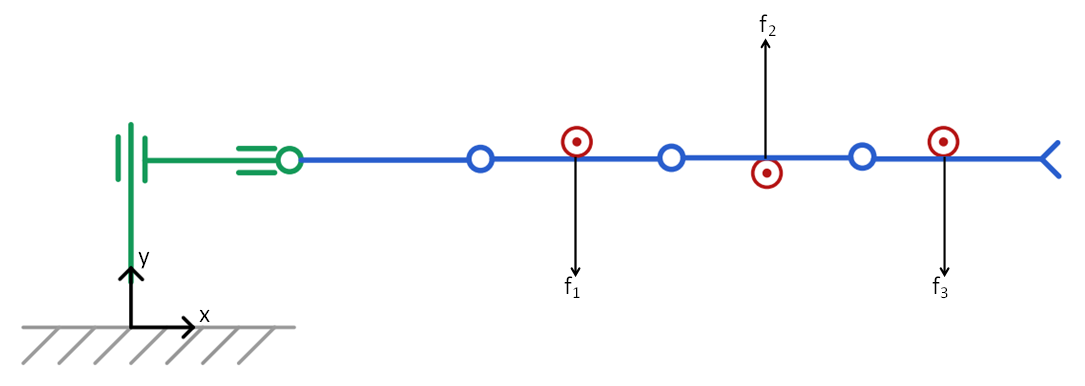
\includegraphics[width=0.8\textwidth]{figures/no_propulsion.PNG}
    \caption{Configuration of the snake robot and obstacles yielding no propulsion}
    \label{fig:noprop}
\end{figure}

In other words there is a subspace of the force space which will not contribute to propulsion. Stavdahl \cite{StavdahlNote} denotes this as the \textbf{constraint space} $\mathbb{C}$. The subspace within which forward motion of the head is achieved is denoted the \textbf{propulsion space} $\mathbb{P}$. The remaining subspace, the \textbf{shape space} $\mathbb{S}$, is the space in which the joint torques simply change the shape configuration of the robot.

Finally, knowledge about the specified spaces may be exploited in planning of a path from one point to another. In particular, it can be used to design an optimal path that maximizes the propulsion space. When the corresponding optimal forces are known, HPFC can be used to realise these forces while adjusting the shape of the robot to the path.

%---------------------------------------------------------------------------------------
%---------------------------------------------------------------------------------------
%---------------------------------------------------------------------------------------

\section{Projection onto path}\label{sec:pathproj}
In order for the robot to adjust its shape to fit the desired path, its controller is dependent on knowing the joint angles that fulfill this task. The desired joint angles are found by projecting the joints of the snake onto the predefined path. It is assumed that the 2D path is known at all times. Since the path has no width it is possible to simply find the shortest distance from a joint to the path to determine where the joint \textit{should have} been. This distance, commonly known as the cross track error, is called $BC$ and is illustrated in Figure \ref{fig:path_proj}. The path can be discretized to consist of points along the lines and curves defining the path.

\begin{figure}[h!]
    \centering
    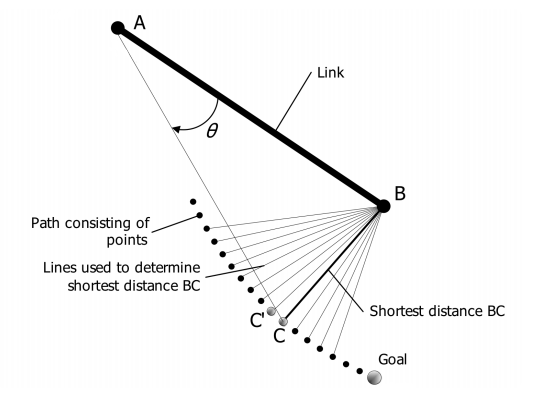
\includegraphics[width=0.7\textwidth]{figures/path_proj.PNG}
    \caption{Shortest distance from joint to path \cite{conkur2008path}}
    \label{fig:path_proj}
\end{figure}

The shortest distance is chosen by numerically comparing all the line segments from the joint to a piece of the path seen as relevant based on the position of the robot. When this point is known, the deviation angle $\theta$ can be determined by trigonometrical properties. The distance $AB$ will equal the length of a link $l$, and the points $A$ and $B$ are respectively the positions of the preceding joint and joint to be projected. The distance $AC$ is now called $a$ and the distance $BC$ is called $b$. The relationship in \ref{eq:lawcos} is given from the law of cosine.

\begin{equation}\label{eq:lawcos}
    \cos{(\theta)} = \frac{l^2 + a^2 - b^2}{2lb}.
\end{equation}
\\
Note that this expression will be invalid if the shortest distance from the joint to the path is zero, meaning the joint is already on the path. There is however no need to perform a projection if there is no deviation from the path. In the case of very precise calculation, the joint and the path will never overlap completely. One can however introduce a very small width around the path in which the joint is considered to be on the path. This is equivalent to the threshold introduced in \cite{conkur2008path}, where an angle deviation $\theta$ lower than a given threshold is ignored.

%The angle $\theta$ is the deviation from the path an thus the joint angle error.
Because no explicit information about which side (left/right) of the path the joints are lying on is assumed, the sign of $\theta$ is unfamiliar. The easiest way to solve this in a computer program is simply comparing the result of rotation around $A$ with both the positive and negative angle options. The link $AB$ is rotated using the rotation matrix $\mathbf{R_z}$, expressed in (\ref{eq:trans_rot}). The resulting projected points are thus

\begin{equation}
    C^+ = A + \mathbf{R_z}(\theta)AB \quad \text{and} \quad
    C^- = A + \mathbf{R_z}(-\theta)AB.
\end{equation}
\\
The angle with the corresponding point closest to $C$ is finally chosen and added to the actual angle of the joint to obtain the new desired angle.


%-----------------------------------------------------------------------------------
%-----------------------------------------------------------------------------------
%-----------------------------------------------------------------------------------

\section{Contact detection}

Before the consequence of an interaction is calculated, the point of contact (if any) has to be determined. This is done by projecting the obstacle point onto the closest link. The distance from the obstacle to the projected point is then compared to the safety radius $r_{safety}$ around each obstacle. This safety radius is to avoid the scenario in which the robot in a discrete time step moves to the opposite side of the obstacle point. Consequently, the relation in (\ref{eq:obstrad}) is obtained. 

\begin{equation}\label{eq:obstrad}
    \text{contact} =
    \begin{cases}
        1 & \text{if $pc \leq r_{safety}$}\\
        0 & \text{else}
    \end{cases}
\end{equation}
\\
Figure \ref{fig:obstrad} shows a case in which contact is established. If link $i$ is considered in contact with an obstacle, the distance $d_{c,i}$, which is a generalized coordinate introduced in \ref{seq:constr_kin}, equals $|AP|$.

\begin{figure}
    \centering
    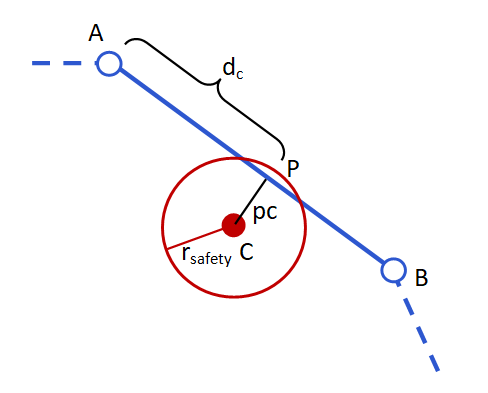
\includegraphics[trim=1cm 1cm 1.2cm 0.6cm, clip=true, width=0.4\textwidth]{figures/obst_radius.PNG}
    \caption{Robot link and obstacle with safety radius}
    \label{fig:obstrad}
\end{figure}


